\documentclass[../mathNotesPreamble]{subfiles}
\begin{document}
%\relscale{1.4}
\section{2.5: Limits at Infinity} 
      \begin{defn*}
        \textbf{Limits at Infinity and Horizontal Asymptotes} 

          If $f(x)$ becomes arbitrarily close to a finite number $L$ for all sufficiently large and positive $x$, then we write
            $$\lim_{x \to \infty} f(x)=L$$
          We say the limit of $f(x)$ as $x$ approaches infinity is $L$. In this case, the line $y=L$ is a \textbf{horizontal asymptote} of $f$. The limit at negative infinity, 
            $$\lim_{x \to -\infty} f(x)=M$$
          is defined analogously. When this limit exists, $y=M$ is a horizontal asymptote.
      \end{defn*}
      \begin{enumerate}[label=]
        \item\textit{Note:} The function \textit{can} cross it's horizontal asymptote (consider $\frac{\sin x}{x}$).
        \item\textit{Note:} A function can have 0, 1 or 2 horizontal asymptotes.
      \end{enumerate}
      
      \begin{ex*}
        For each of the following functions, find $\ds\lim_{x \to \infty} f(x)$ and $\ds\lim_{x \to -\infty} f(x)$.
      \end{ex*}
      \begin{tasks}(2)
        \task $f(x)=\dfrac{1}{x^2}$
        \task $f(x)=\dfrac{1}{x^3}$
      \end{tasks}
        \pagebreak
      \begin{tasks}[resume, after-item-skip=\stretch{1}](2)
        \task $f(x)=2+\dfrac{10}{x^2}$
        \task $f(x)=5+\dfrac{\sin x}{\sqrt x}$
        \task $f(x)=\parens{5+\dfrac{1}{x}+\dfrac{10}{x^2}}$
        \task $f(x)=\parens{3x^{12}-9x^7}$
        \task $f(x)=\sin(x)$
        \task $f(x)=\dfrac{\sin x}{x}$
      \end{tasks}
      \vspace*{\stretch{1}}
      \pagebreak
      \begin{defn*}
        \textbf{Infinite Limits at Infinity}
        If $f(x)$ becomes arbitrarily large as $x$ becomes arbitrarily large, then we write
          $$\lim_{x \to \infty} f(x)=\infty$$
        The limits $\ds\lim_{x \to \infty}=-\infty,\ds\lim_{x \to -\infty}=\infty$ and $\ds\lim_{x \to -\infty}=-\infty$ are defined similarly.
      \end{defn*}
      \begin{center}
        \begin{tikzpicture}[scale=0.9]
          \begin{groupplot}[
            group style={group size=2 by 2, horizontal sep=2cm, vertical sep=2.2cm},
            axis lines=center, 
            axis line style={->},
            xmin=-4.5, xmax=4.5,
            ymin=-5, ymax=40,
            ymajorticks=false,
            every axis plot/.append style={line width=0.95pt},
            ylabel=Even functions, ylabel style={at={(ticklabel* cs:1.1)},anchor=south},
            ]
          \nextgroupplot
            \addplot[<->] expression[domain=-4.5:4.5, blue, samples=50] {x^2};
            \addplot[<->] expression[domain=-2.52:2.52, red, samples=50] {x^4};
            \addplot[<->] expression[domain=-1.85:1.85, black, samples=50] {x^6};
          \nextgroupplot[
            ymin=-40, ymax=40,
            ylabel=Odd functions
            ]
            \addplot[<->] expression[domain=-3.4:3.4, blue, samples=50] {x^3};
            \addplot[<->] expression[domain=-2.09:2.09, red, samples=50] {x^5};
            \addplot[<->] expression[domain=-1.69:1.69, black, samples=50] {x^7};
          \nextgroupplot[
            ymin=-5, ymax=40,
            ylabel=$1/x^n:\ n$ Even
            ]
            \addplot[<->] expression[domain=-4.5:-0.158, blue, samples=50] {x^(-2)};
            \addplot[<->] expression[domain=0.158:4.5, blue, samples=50] {x^(-2)};
            \addplot[<->] expression[domain=-4.5:-0.3976, red, samples=50] {x^(-4)};
            \addplot[<->] expression[domain=0.3976:4.5, red, samples=50] {x^(-4)};
            \addplot[<->] expression[domain=-4.5:-0.541, black, samples=50] {x^(-6)};
            \addplot[<->] expression[domain=0.541:4.5, black, samples=50] {x^(-6)};
          \nextgroupplot[
            ymin=-40, ymax=40,
            ylabel=$1/x^n:\ n$ Odd
            ]
            \addplot[<->] expression[domain=-4.5:-0.2924, blue, samples=50] {x^(-3)};
            \addplot[<->] expression[domain=0.2924:4.5, blue, samples=50] {x^(-3)};
              \addlegendentry{$1/x^3$};
            \addplot[<->] expression[domain=-4.5:-0.4782, red, samples=50] {x^(-5)};
            \addplot[<->] expression[domain=0.4782:4.5, red, samples=50] {x^(-5)};
              \addlegendentry{$1/x^5$};
            \addplot[<->] expression[domain=-4.5:-0.5904, black, samples=50] {x^(-7)};
            \addplot[<->] expression[domain=0.5904:4.5, black, samples=50] {x^(-7)};
              \addlegendentry{$1/x^7$};
          \end{groupplot}
        \end{tikzpicture}
      \end{center}
      \pagebreak

      \begin{thmBox*}[Theorem 2.6: Limits at Infinity of Powers and Polynomials]
        Let $n$ be a positive integer and let $p$ be the polynomial 
          $$p(x)=a_nx^n+a_\nmo x^\nmo+\cdots+a_2x^2+a_1x+a_0, \text{ where } a_n\neq 0.$$
        \begin{enumerate}
          \item $\ds\lim_{x \to \pm \infty} x^n=\infty$ when $n$ is even.
          \item $\ds\lim_{x \to \infty} x^n=\infty$ and $\ds\lim_{x \to -\infty} x^n=-\infty$ when $n$ is odd.
          \item $\ds\lim_{x \to \pm\infty} \dfrac{1}{x^n}=\ds\lim_{x \to \pm\infty}x\inv[n]=0$.
          \item $\ds\lim_{x \to \pm\infty} p(x)=\lim_{x \to \pm\infty} a_nx^n=\pm\infty$, depending on the degree of the polynomial and the sign of the leading coefficient $a_n$.
        \end{enumerate}
      \end{thmBox*}

      \begin{enumerate}[label=]
        \item \textit{Note:} All previous limit laws still apply (e.g. constant multiplier rule)
        \item \textit{Note:} This theorem \textit{ONLY} applies for $x\to\pm\infty$. When $x\to a, \abs{a}<\infty$, we compute the left and right limits and use sm+/sm- (as done in section 2.4).
      \end{enumerate}
      \begin{ex*}
        For the following, find the limits as $x\to-\infty$ and $x\to \infty$:
        \begin{tasks}[after-item-skip=\stretch{1}](2)
          \task[] $f(x)=2x\inv[8]$
          \task[] $g(x)=-12x\inv[5]$
          \task[] $h(x)=3x^{12}-9x^7$
          \task[] $\ell(x)=2x\inv[8]+4x^3$
        \end{tasks}
        \vspace*{\stretch{1}}
      \end{ex*}
      \pagebreak 
      
      When finding the limit as $x\to\pm\infty$ of a rational function, $\frac{p(x)}{q(x)}$, where $p(x)$ and $q(x)$ are polynomial functions, we multiply the function by $\dfrac{\sfrac{1}{x^n}}{\sfrac{1}{x^n}}$, where $n$ is the highest degree in the denominator $q(x)$.
      
      \textit{Note:} To receive full credit for questions of this type, you must show all the fractions in your intermediate steps.
      \begin{ex*}\ 
      
        \begin{tasks}(1)
          \task $\ds\lim_{x \to \infty}\dfrac{1-x}{2x}$\\[50pt]
          \task $\ds\lim_{x \to \infty}\dfrac{1-x}{x^2}$\\[50pt]
          \task $\ds\lim_{x \to \infty}\dfrac{1-x^2}{2x}$
        \end{tasks}
      \end{ex*}
      \pagebreak
      
      \begin{thmBox*}[Theorem 2.7: End Behavior and Asymptotes of Rational Functions]
        Suppose $f(x)=\dfrac{p(x)}{q(x)}$ is a rational function, where 
          \begin{align*}
            p(x)&= a_mx^m+a_\mmo x^\mmo+\cdots+a_2x^2+a_1x+a_0\\
            q(x)&= b_nx^n+b_\nmo x^\nmo+\cdots+b_2x^2+b_1x+b_0
          \end{align*}
        with $a_m\neq0$ and $b_n\neq 0$.
        \begin{enumerate}
          \item \textbf{Degree of numerator less than degree of denominator}

          If $m<n$, then $\lim_{x \to \pm\infty} f(x)=0$ and $y=0$ is a horizontal asymptote of $f$.
          \item \textbf{Degree of numerator equals degree of denominator}

          If $m=n$, then $\lim_{x \to \pm\infty} f(x)=a_m/b_n$ and $y=a_m/b_n$ is a horizontal asymptote of $f$.
          \item \textbf{Degree of numerator greater than degree of denominator}

          If $m>n$, then $\lim_{x \to \pm\infty} f(x)=\infty$ or $-\infty$ and $f$ has no horizontal asymptote.
          \item \textbf{Slant Asymptote}

          If $m=n+1$, then $\lim_{x \to \pm \infty}f(x)=\infty$ or $-\infty$, and $f$ has no horizontal asymptote, but $f$ has a slant asymptote.
          \item \textbf{Vertical asymptotes}

          Assuming $f$ is in reduced form ($p$ and $q$ share no common factors), vertical asymptotes occur at the zeros of $q$.
          \end{enumerate}
      \end{thmBox*}
      \pagebreak
      
      \begin{ex*}
        Evaluate the limits of the following as $x\to-\infty$ and $x\to\infty$. State the equation of the horizontal asymptote.
        \begin{enumerate}
          \item $f(x)=\dfrac{2x^3+7}{x^3-x^2+x+7}$
            \vspace*{\stretch{1}}
          \item $g(x)=\dfrac{1}{x^3-4x+1}$
            \vspace*{\stretch{1}}
          \item $h(x)=\dfrac{3x^5+2x^2-2}{4x^4-3x}$
            \vspace*{\stretch{1}}
          \item $j(x)=\dfrac{4x^2-2x+3}{7x^2-1}$
            \vspace*{\stretch{1}}
          \item $\ell(x)=\dfrac{1-x^2}{3+2x-x^3}$
            \vspace*{\stretch{1}}
        \end{enumerate}
      \end{ex*}
      \pagebreak
      
      \begin{defn*}
      When the degree of the numerator, $m$, is greater than the degree of the denominator, $n$, the function has an oblique asymptote:
        $$f(x)=\dfrac{p(x)}{q(x)}=a(x)+\dfrac{r(x)}{q(x)}$$
      where $a(x)$ is the resulting polynomial that we get from polynomial long division and $r(x)$ is the remainder. We are interested in the special case where $m=n+1$, and $f(x)$ has a \textbf{slant asymptote}.
      \end{defn*}
      \begin{ex*}
        For the following functions, find the vertical asymptotes and the slant asymptotes:
      \end{ex*}
      \begin{enumerate}[itemsep=\stretch{1}]
        \item $y=\dfrac{2x^3+x^2+x+3}{x^2+2x}$
        \item $f(x)=\dfrac{x^2-1}{x+2}$
      \end{enumerate}
      \vspace*{\stretch{1}}
      \pagebreak
      \begin{enumerate}[itemsep=\stretch{1}]
        \setcounter{enumi}{2}
        \item $g(t)=\dfrac{t^2-1}{2t+4}$
        \item $h(u)=\dfrac{u^2}{u-1}$
      \end{enumerate}
      \vspace*{\stretch{1}}
      \pagebreak
      If the denominator has a square root, we need to change our work depending on if $x\to-\infty$ or $x\to\infty$:\\
      
      \begin{ex*}
        For the following, find the equation of the horizontal asymptotes:
        
      \noindent
      \begin{minipage}[t]{0.5\linewidth}
          \vspace*{20pt}
          \begin{tasks}[after-item-skip=0.10\paperheight](1)
            \task $\ds\lim_{x \to \infty}\dfrac{x}{\sqrt{x^2+3}}$
            \task $\ds\lim_{x \to-\infty}\dfrac{x}{\sqrt{x^2+3}}$
            \task $\ds\lim_{x \to \infty}\dfrac{x}{\sqrt{x^2+x}}$
            \task $\ds\lim_{x \to-\infty}\dfrac{x}{\sqrt{x^2+x}}$
          \end{tasks}
      \end{minipage}%
      \begin{minipage}[t]{0.5\linewidth}\ 
      
        \begin{flushright}
          \begin{tikzpicture}
            \begin{axis}[
              axis lines=center,
              axis line style={->},
              xmin=-6.5, xmax=6.5,
              ymin=-2.25, ymax=2.25,
              ticklabel style={font=\tiny,inner sep=0.75pt,fill=white},
              xlabel=$x$, xlabel style={at={(ticklabel* cs:1)},anchor=north west},
              ylabel=$y$, ylabel style={at={(ticklabel* cs:1)},anchor=south west},
              every axis plot/.append style={line width=0.95pt},
              legend style={at={(axis cs:1.25,-1.5)},draw=none,anchor=south west},
              ]
              \addplot[<->] expression[domain=-6:6, blue] {x/(sqrt(x^2+3)};
                \addlegendentry{$\frac{x}{\sqrt{x^2+3}}$};
            \end{axis}
          \end{tikzpicture}
        \end{flushright}
      \end{minipage}%
      \end{ex*}
      \vspace*{\stretch{1}}
      \pagebreak
      \begin{tasks}[resume, after-item-skip=0.2\paperheight](1)
        \task $\dfrac{7x^3-2}{-x^3+\sqrt{25x^6+4}}$
        \task $\dfrac{\sqrt[3]{x^6+8}}{4x^2+\sqrt{3x^4+1}}$
        \task $\dfrac{2x}{\sqrt{x^2-x-2}}$
      \end{tasks}
      \pagebreak
      
      \begin{ex*}
        For the following, sketch a graph with the following properties:
        
        \noindent
        \begin{minipage}[t]{0.35\linewidth}\ 
        
          \begin{enumerate}
            \item 
              \begin{enumerate}[label=]
                \itemsep10pt 
                \item $\ds\lim_{x \to 0} f(x)=-\infty$
                \item $\ds\lim_{x \to 2} f(x)=\dfrac{5}{4}$
                \item $\ds\lim_{x \to \pm\infty} f(x)=1$
                \item $f(2)$ DNE
                \item $f(1)=1$
                \item $f(-1)=-1$
              \end{enumerate}
          \end{enumerate}
          
        \end{minipage}%
        \begin{minipage}[t]{0.65\linewidth}\ 
          \begin{flushright}
            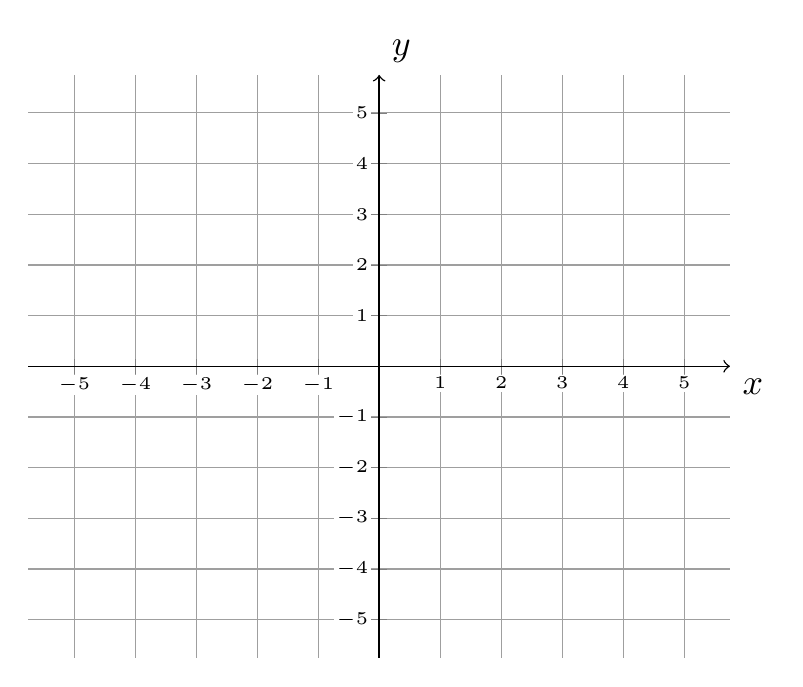
\begin{tikzpicture}[scale=1.3]
              \begin{axis}[
                grid=both,
                grid style={line width=0.35pt, draw=gray!75},
                axis lines=center,
                axis line style={->},
                xmin=-5, xmax=5,
                ymin=-5, ymax=5,
                xtick={-5,-4,...,5},
                ytick={-5,-4,...,6},
                enlargelimits={abs=0.75},
                ticklabel style={font=\tiny,inner sep=0.75pt,fill=white},
                xlabel=$x$, xlabel style={at={(ticklabel* cs:1)},anchor=north west},
                ylabel=$y$, ylabel style={at={(ticklabel* cs:1)},anchor=south west},
                every axis plot/.append style={line width=0.95pt}
                ]
              \end{axis}
            \end{tikzpicture}
          \end{flushright}
        \end{minipage}
        
        \vspace*{\stretch{1}}
        \noindent
        \begin{minipage}[t]{0.35\linewidth}\ 
        
          \begin{enumerate}
            \setcounter{enumi}{1}
            \item 
              \begin{enumerate}[label=]
                \itemsep10pt 
                \item $\ds\lim_{x \to -1^-} f(x)=\infty$
                \item $\ds\lim_{x \to -1^+} f(x)=-\infty$
                \item $\ds\lim_{x \to \pm\infty} f(x)=2$
                \item $f(0)=-2$
                \item $f(1)=1$
                \item $f(-2)=4$
              \end{enumerate}
          \end{enumerate}
          
        \end{minipage}%
        \begin{minipage}[t]{0.65\linewidth}\ 
        
          \begin{flushright}
            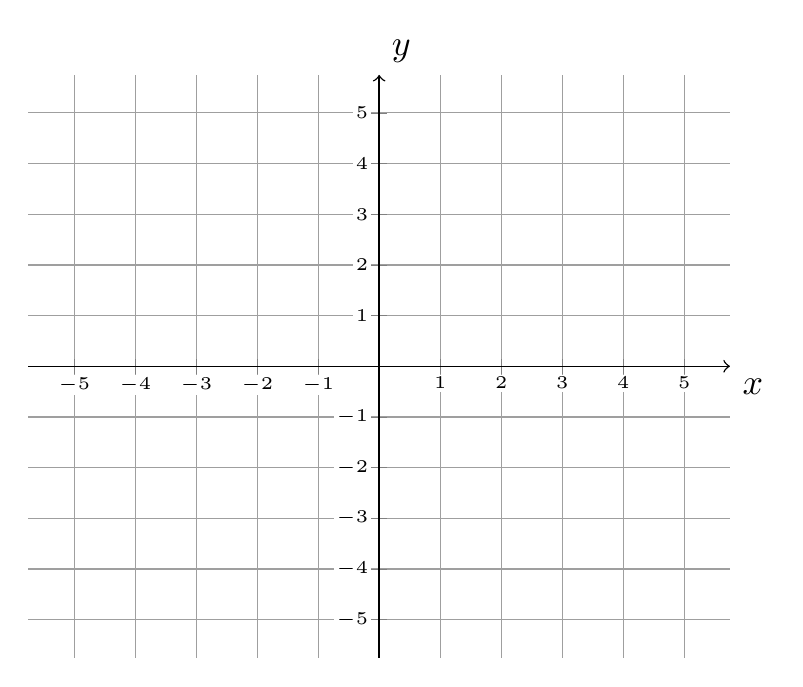
\begin{tikzpicture}[scale=1.3]
              \begin{axis}[
                grid=both,
                grid style={line width=0.35pt, draw=gray!75},
                axis lines=center,
                axis line style={->},
                xmin=-5, xmax=5,
                ymin=-5, ymax=5,
                xtick={-5,-4,...,5},
                ytick={-5,-4,...,6},
                enlargelimits={abs=0.75},
                ticklabel style={font=\tiny,inner sep=0.75pt,fill=white},
                xlabel=$x$, xlabel style={at={(ticklabel* cs:1)},anchor=north west},
                ylabel=$y$, ylabel style={at={(ticklabel* cs:1)},anchor=south west},
                every axis plot/.append style={line width=0.95pt}
                ]
              \end{axis}
            \end{tikzpicture}
          \end{flushright}
        \end{minipage}
      \end{ex*}
      \pagebreak
      
      \begin{ex*}
        Find \textit{all} asymptotes (vertical, horizontal, slant)
        \begin{enumerate}
          \item $\dfrac{x^3-10x^2+16x}{x^2-8x}$
            \vspace*{\stretch{1}}
          \item $\dfrac{\cos x+2\sqrt x}{\sqrt x}$
            \vspace*{\stretch{1}}
        \end{enumerate}
      \end{ex*}
      \pagebreak
      
      Other function end behavior to consider include $e^x, e\inv[x], \ln(x)$ and $\tan\inv(x)$:
      \begin{center}
        \begin{tikzpicture}
          \begin{groupplot}[
            group style={group size=2 by 2, horizontal sep=2cm, vertical sep=2cm},
            axis lines=center,
            axis line style={->},
            xmin=-6.5, xmax=6.5,
            ymin=-2.25, ymax=6.5,
            ticklabel style={font=\tiny,inner sep=0.75pt,fill=white},
            xlabel=$x$, xlabel style={at={(ticklabel* cs:1)},anchor=north west},
            ylabel=$y$, ylabel style={at={(ticklabel* cs:1)},anchor=south west},
            every axis plot/.append style={line width=0.95pt},
            legend style={at={(axis cs:6,-2)},anchor=south east},
            ]
          \nextgroupplot
            \addplot[<->] expression[domain=-6:1.8, blue, samples=100] {e^x};
              \addlegendentry{$e^x$};
          \nextgroupplot
            \addplot[<->] expression[domain=-1.8:6, blue, samples=100] {e^(-x)};
              \addlegendentry{$e\inv[x]$};
          \nextgroupplot[
            xmin=-0.5, xmax=8.5,
            ymin=-4.5, ymax=4.5,
            legend style={at={(axis cs:8,-4)},anchor=south east},
            ]
            \addplot[<->] expression[domain=0.0111:8, samples=500, blue] {ln(x)};
              \addlegendentry{$\ln(x)$};
          \nextgroupplot[
            xmin=-6.5, xmax=6.5,
            ymin=-2.25, ymax=2.25,
            legend style={at={(axis cs:6,-2)},anchor=south east},
            ]
            \addplot[<->] expression[domain=-6.45:6.45, samples=500, blue] {rad(atan(x))};
              \addlegendentry{$\tan\inv(x)$};
          \end{groupplot}
        \end{tikzpicture}
      \end{center}
      \vspace*{\stretch{0.2}}
      \begin{tasks}[after-item-skip=\stretch{1}](2)
        \task $\ds\lim_{x \to -\infty}\sin x$
        \task $\ds\lim_{x \to \infty}\sin x$
        \task $\ds\lim_{x \to -\infty}\cos x$
        \task $\ds\lim_{x \to \infty}\cos x$
      \end{tasks}
      \vspace*{\stretch{1}}
      \pagebreak
\end{document}
